% Copyright 2004 by Till Tantau <tantau@users.sourceforge.net>.
%
% In principle, this file can be redistributed and/or modified under
% the terms of the GNU Public License, version 2.
%
% However, this file is supposed to be a template to be modified
% for your own needs. For this reason, if you use this file as a
% template and not specifically distribute it as part of a another
% package/program, I grant the extra permission to freely copy and
% modify this file as you see fit and even to delete this copyright
% notice. 

\documentclass{beamer}
\usepackage[utf8]{inputenc}
\usepackage[UKenglish]{babel}
\usepackage{graphicx}
\graphicspath{ {images/} }

%\usepackage{biblatex}
%\addbibresource{presentation.bib}

% There are many different themes available for Beamer. A comprehensive
% list with examples is given here:
% http://deic.uab.es/~iblanes/beamer_gallery/index_by_theme.html
% You can uncomment the themes below if you would like to use a different
% one:
%\usetheme{AnnArbor}
%\usetheme{Antibes}
%\usetheme{Bergen}
%\usetheme{Berkeley}
%\usetheme{Berlin}
%\usetheme{Boadilla}
%\usetheme{boxes}
%\usetheme{CambridgeUS}
%\usetheme{Copenhagen}
%\usetheme{Darmstadt}
%\usetheme{default}
\usetheme{Frankfurt}
%\usetheme{Goettingen}
%\usetheme{Hannover}
%\usetheme{Ilmenau}
%\usetheme{JuanLesPins}
%\usetheme{Luebeck}
%\usetheme{Madrid}
%\usetheme{Malmoe}
%\usetheme{Marburg}
%\usetheme{Montpellier}
%\usetheme{PaloAlto}
%\usetheme{Pittsburgh}
%\usetheme{Rochester}
%\usetheme{Singapore}
%\usetheme{Szeged}
%\usetheme{Warsaw}

\title{Hitchhiker Guide to Hardware Maintenance}

% A subtitle is optional and this may be deleted
% \subtitle{Optional Subtitle}

\author{Hélder Silva}
% - Give the names in the same order as the appear in the paper.
% - Use the \inst{?} command only if the authors have different
%   affiliation.

% - Use the \inst command only if there are several affiliations.
% - Keep it simple, no one is interested in your street address.

\date{Porto Summer of Code, 2016}
% - Either use conference name or its abbreviation.
% - Not really informative to the audience, more for people (including
%   yourself) who are reading the slides online

\subject{Hardware}
% This is only inserted into the PDF information catalog. Can be left
% out. 

% If you have a file called "university-logo-filename.xxx", where xxx
% is a graphic format that can be processed by latex or pdflatex,
% resp., then you can add a logo as follows:

% \pgfdeclareimage[height=0.5cm]{university-logo}{university-logo-filename}
% \logo{\pgfuseimage{university-logo}}

% Delete this, if you do not want the table of contents to pop up at
% the beginning of each subsection:
% \AtBeginSubsection[]
% {
%   \begin{frame}<beamer>{Outline}
%     \tableofcontents[currentsection,currentsubsection]
%   \end{frame}
% }

% Let's get started
\begin{document}

\begin{frame}
  \titlepage
\end{frame}

\begin{frame}{Outline}
  \tableofcontents
  % You might wish to add the option [pausesections]
\end{frame}

\section{What?}

\begin{frame}{Cleaning}
    \begin{itemize}
        \item Remove heat sinks (laptops and desktops)
        \item Clean the fans and air vents
        \item Clean old thermal paste
        \item Apply thermal paste
    \end{itemize}
\end{frame}

\section{Why?}

\subsection{Heat}
\begin{frame}{Heat}
    Dust acts as a thermal insulator and reduces airflow, thereby reducing heat sink and fan performance.
    \newline
    \newline
    Poor heat transfer due to poor thermal contact between components to be cooled and cooling devices.
\end{frame}

\begin{frame}{Dust}
    \centering
    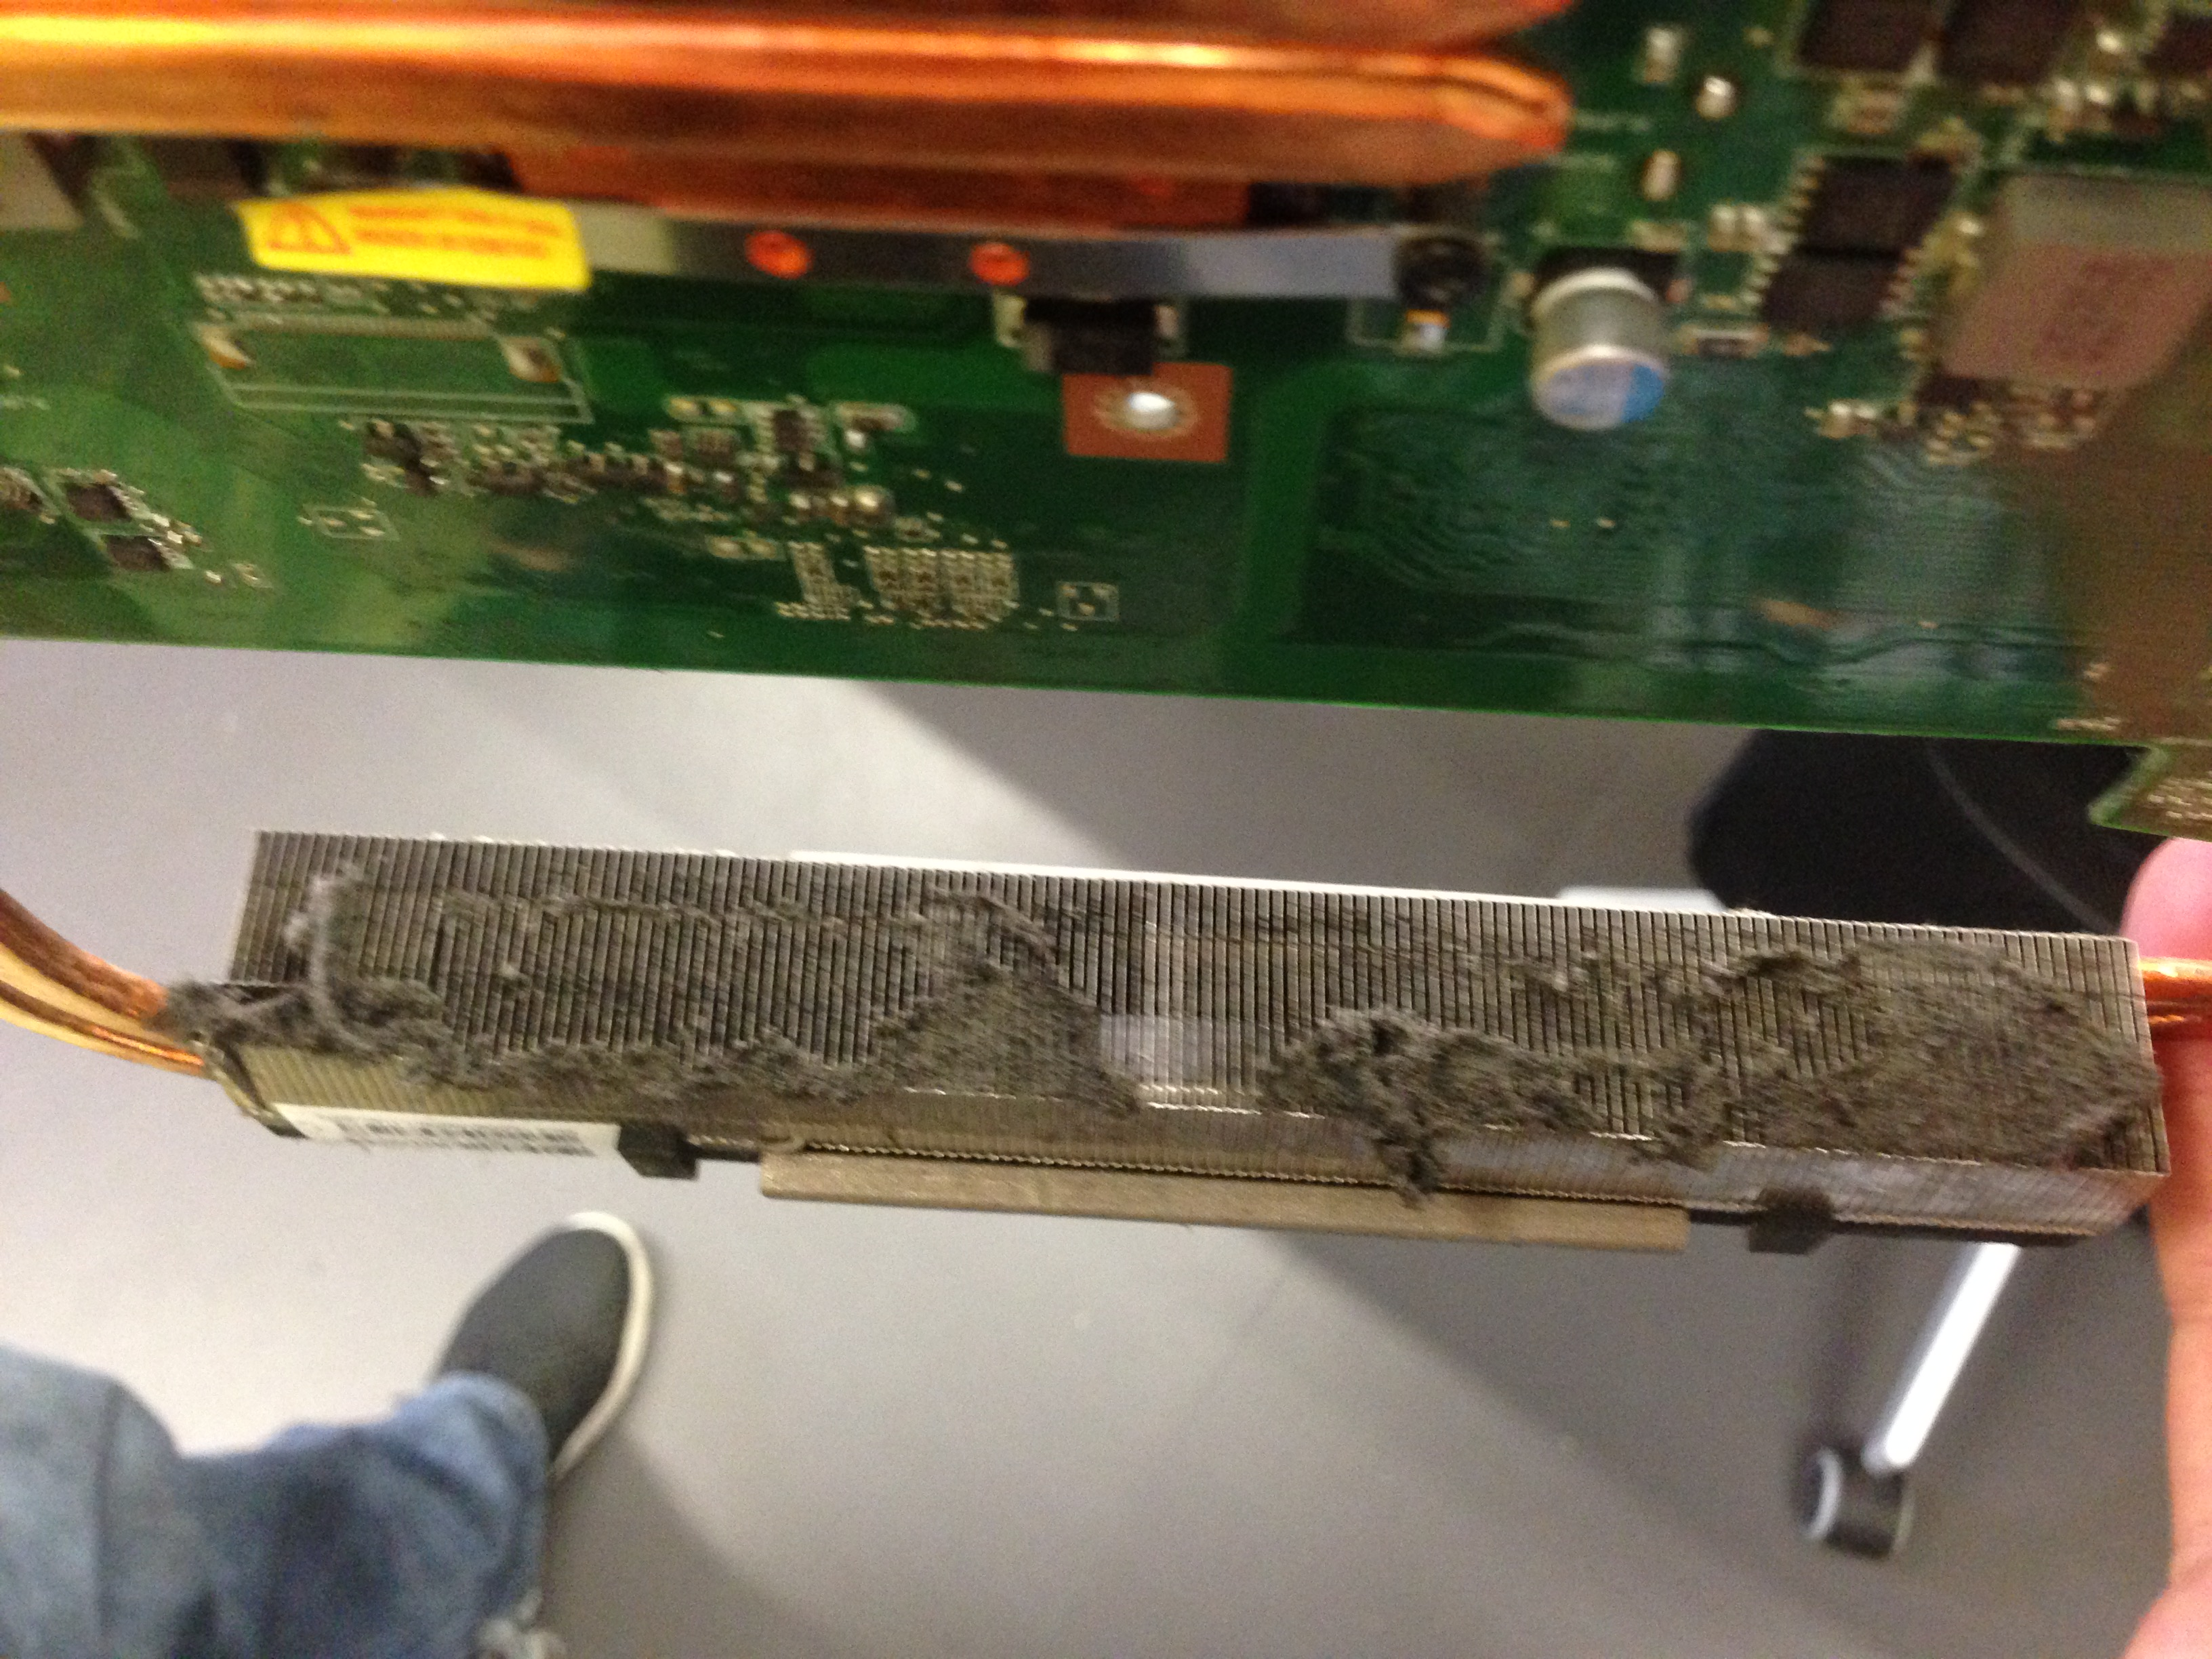
\includegraphics[scale=0.08]{dust}
\end{frame}

\begin{frame}{Dry TIM}
    \centering
    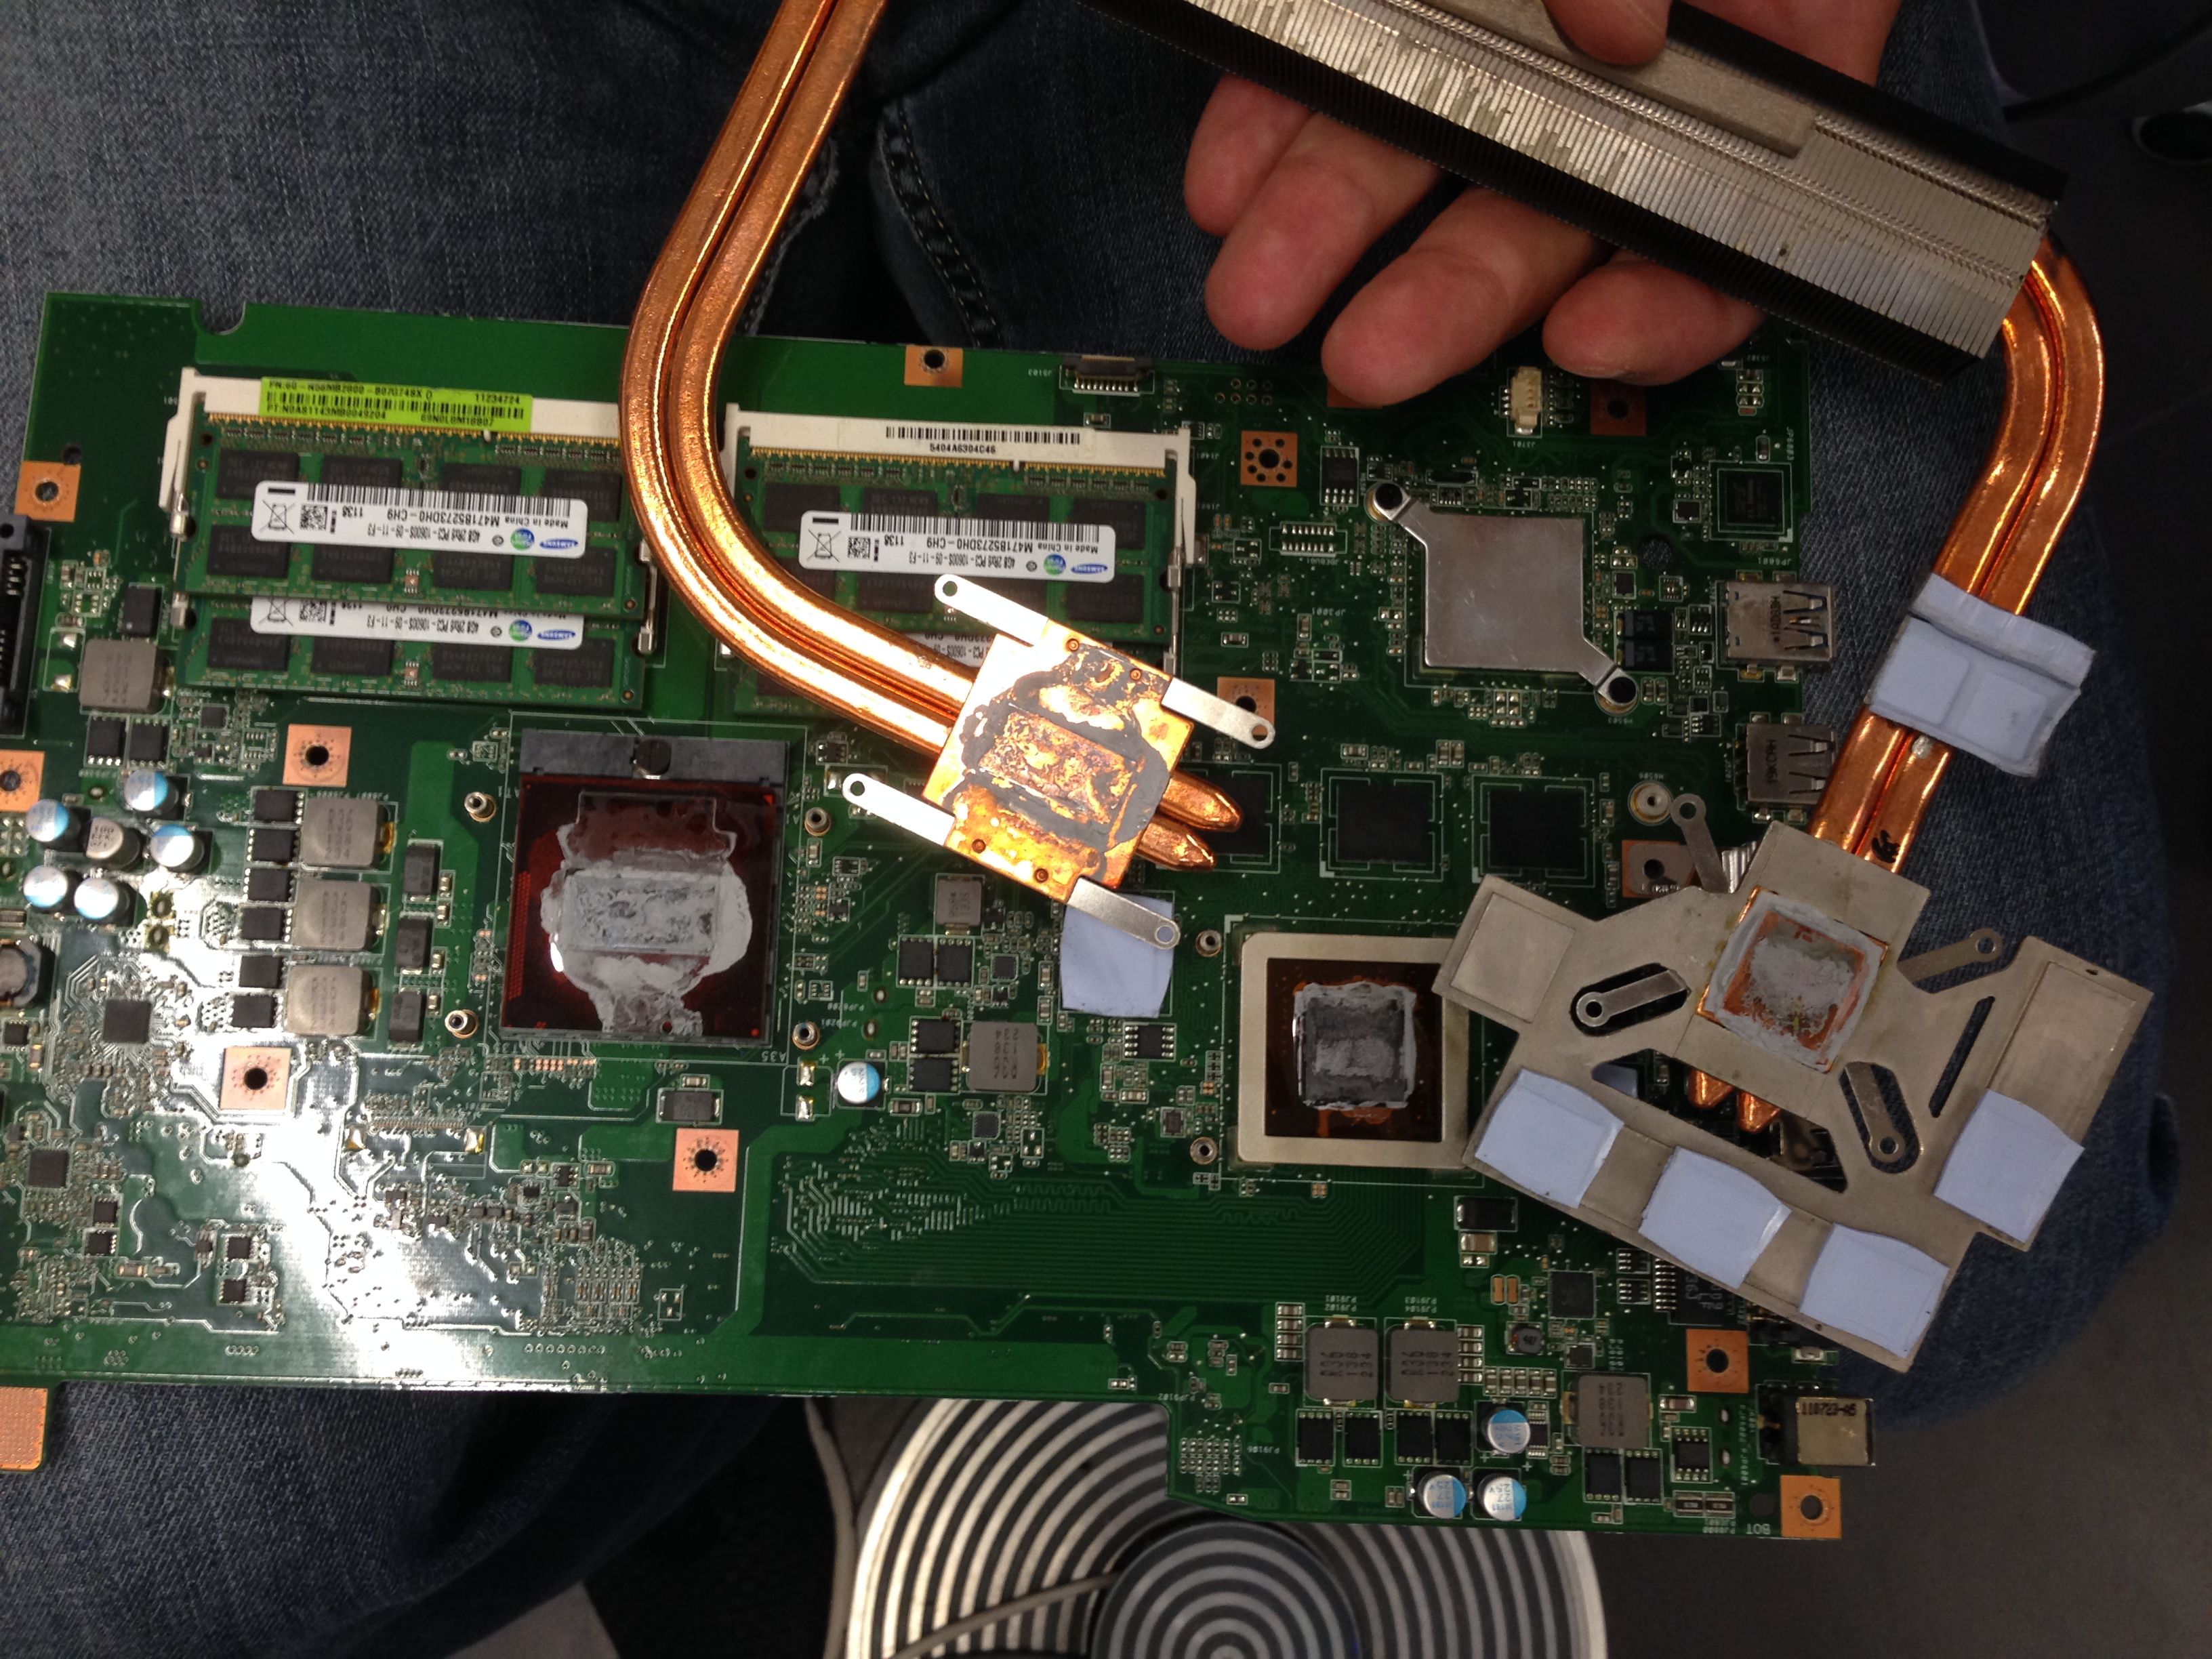
\includegraphics[scale=0.08]{dry-tim}
\end{frame}

\begin{frame}{TIM?}
    \centering
    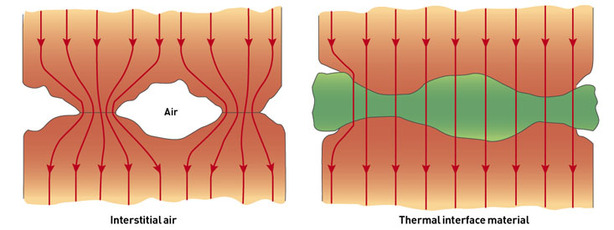
\includegraphics[scale=0.5]{tim-air}
    \newline
    \newline
    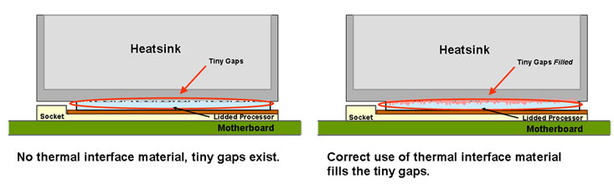
\includegraphics[scale=0.5]{heatsink-tim-cpu}
\end{frame}

\subsection{Throttle}
\begin{frame}{Throttle}
    Because high temperatures can significantly reduce life span or cause permanent damage to components, and the heat output of components can sometimes exceed the computer's cooling capacity, manufacturers often take additional precautions to ensure that temperatures remain within safe limits.
    \newline
    \newline
    Throttling reduces the operating frequency and voltage of an integrated circuit or disables non-essential features of the chip to reduce heat output, often at the cost of slightly or significantly reduced performance.
\end{frame}

\begin{frame}{Damage prevention}
    Most components can shut themselves down when high temperatures are detected to prevent permanent damage.
    \newline
    \newline
    This may not completely guarantee long-term safe operation.
\end{frame}

\section{How?}

\begin{frame}{How?}
    \begin{itemize}
        \item Search for "[model] disassembling" on YouTube/Google
        \item Watch/read the instructions (more than once)
        \item ????
        \item Profit
    \end{itemize}
\end{frame}

\subsection{Tools}

\begin{frame}{Opening}
    \begin{itemize}
        \item Good quality screwdriver
        \item ESD safe gloves
        \item Anti-Static wrist strap
        \item Guitar picks
        \item Tweezers
        \item Magnetic pad (optional)
    \end{itemize}
\end{frame}

\begin{frame}{Cleaning}
    \begin{itemize}
        \item Anti-Static Brush
        \item Dust Blower
        \item Microfiber Cleaning Cloths
    \end{itemize}
\end{frame}

\subsection{Consumables}

\begin{frame}{Consumables}
    \begin{itemize}
      \item Alcohol (70\% solution is enough but the higher the percentage the better)
      \item Cotton swabs/balls
      \item Paper towel
      \item Thermal paste
      \item Thermal pads (optional)
    \end{itemize}
\end{frame}

\subsection{How to}

\begin{frame}{Disassembling}
    \begin{itemize}
      \item Don't use to much pressure on screws
      \item Use small increments of force to open plastic parts
      \item Don't use too much force to remove the heat sinks
      \item Place your screws (and every that comes out of the laptop) in a secure place
    \end{itemize}
    \begin{alertblock}{Important}
        Hardware is always right
    \end{alertblock}
\end{frame}

\begin{frame}{Cleaning}
    \begin{itemize}
        \item Use paper towels to remove the majority of old TIM
        \item Use a non-abrasive (soft plastic) spatula to remove "glued" TIM
        \item Use the cotton/swabs to completely clean the heat sink and circuit
        \item Check if any cleaning material is left on the parts
    \end{itemize}
    \begin{alertblock}{Important}
        Be careful removing the old TIM
    \end{alertblock}
    \begin{alertblock}{Important}
        Try to save the thermal pads
    \end{alertblock}
\end{frame}

\subsection{Examples}

\begin{frame}{Cleaned Dust}
    \centering
    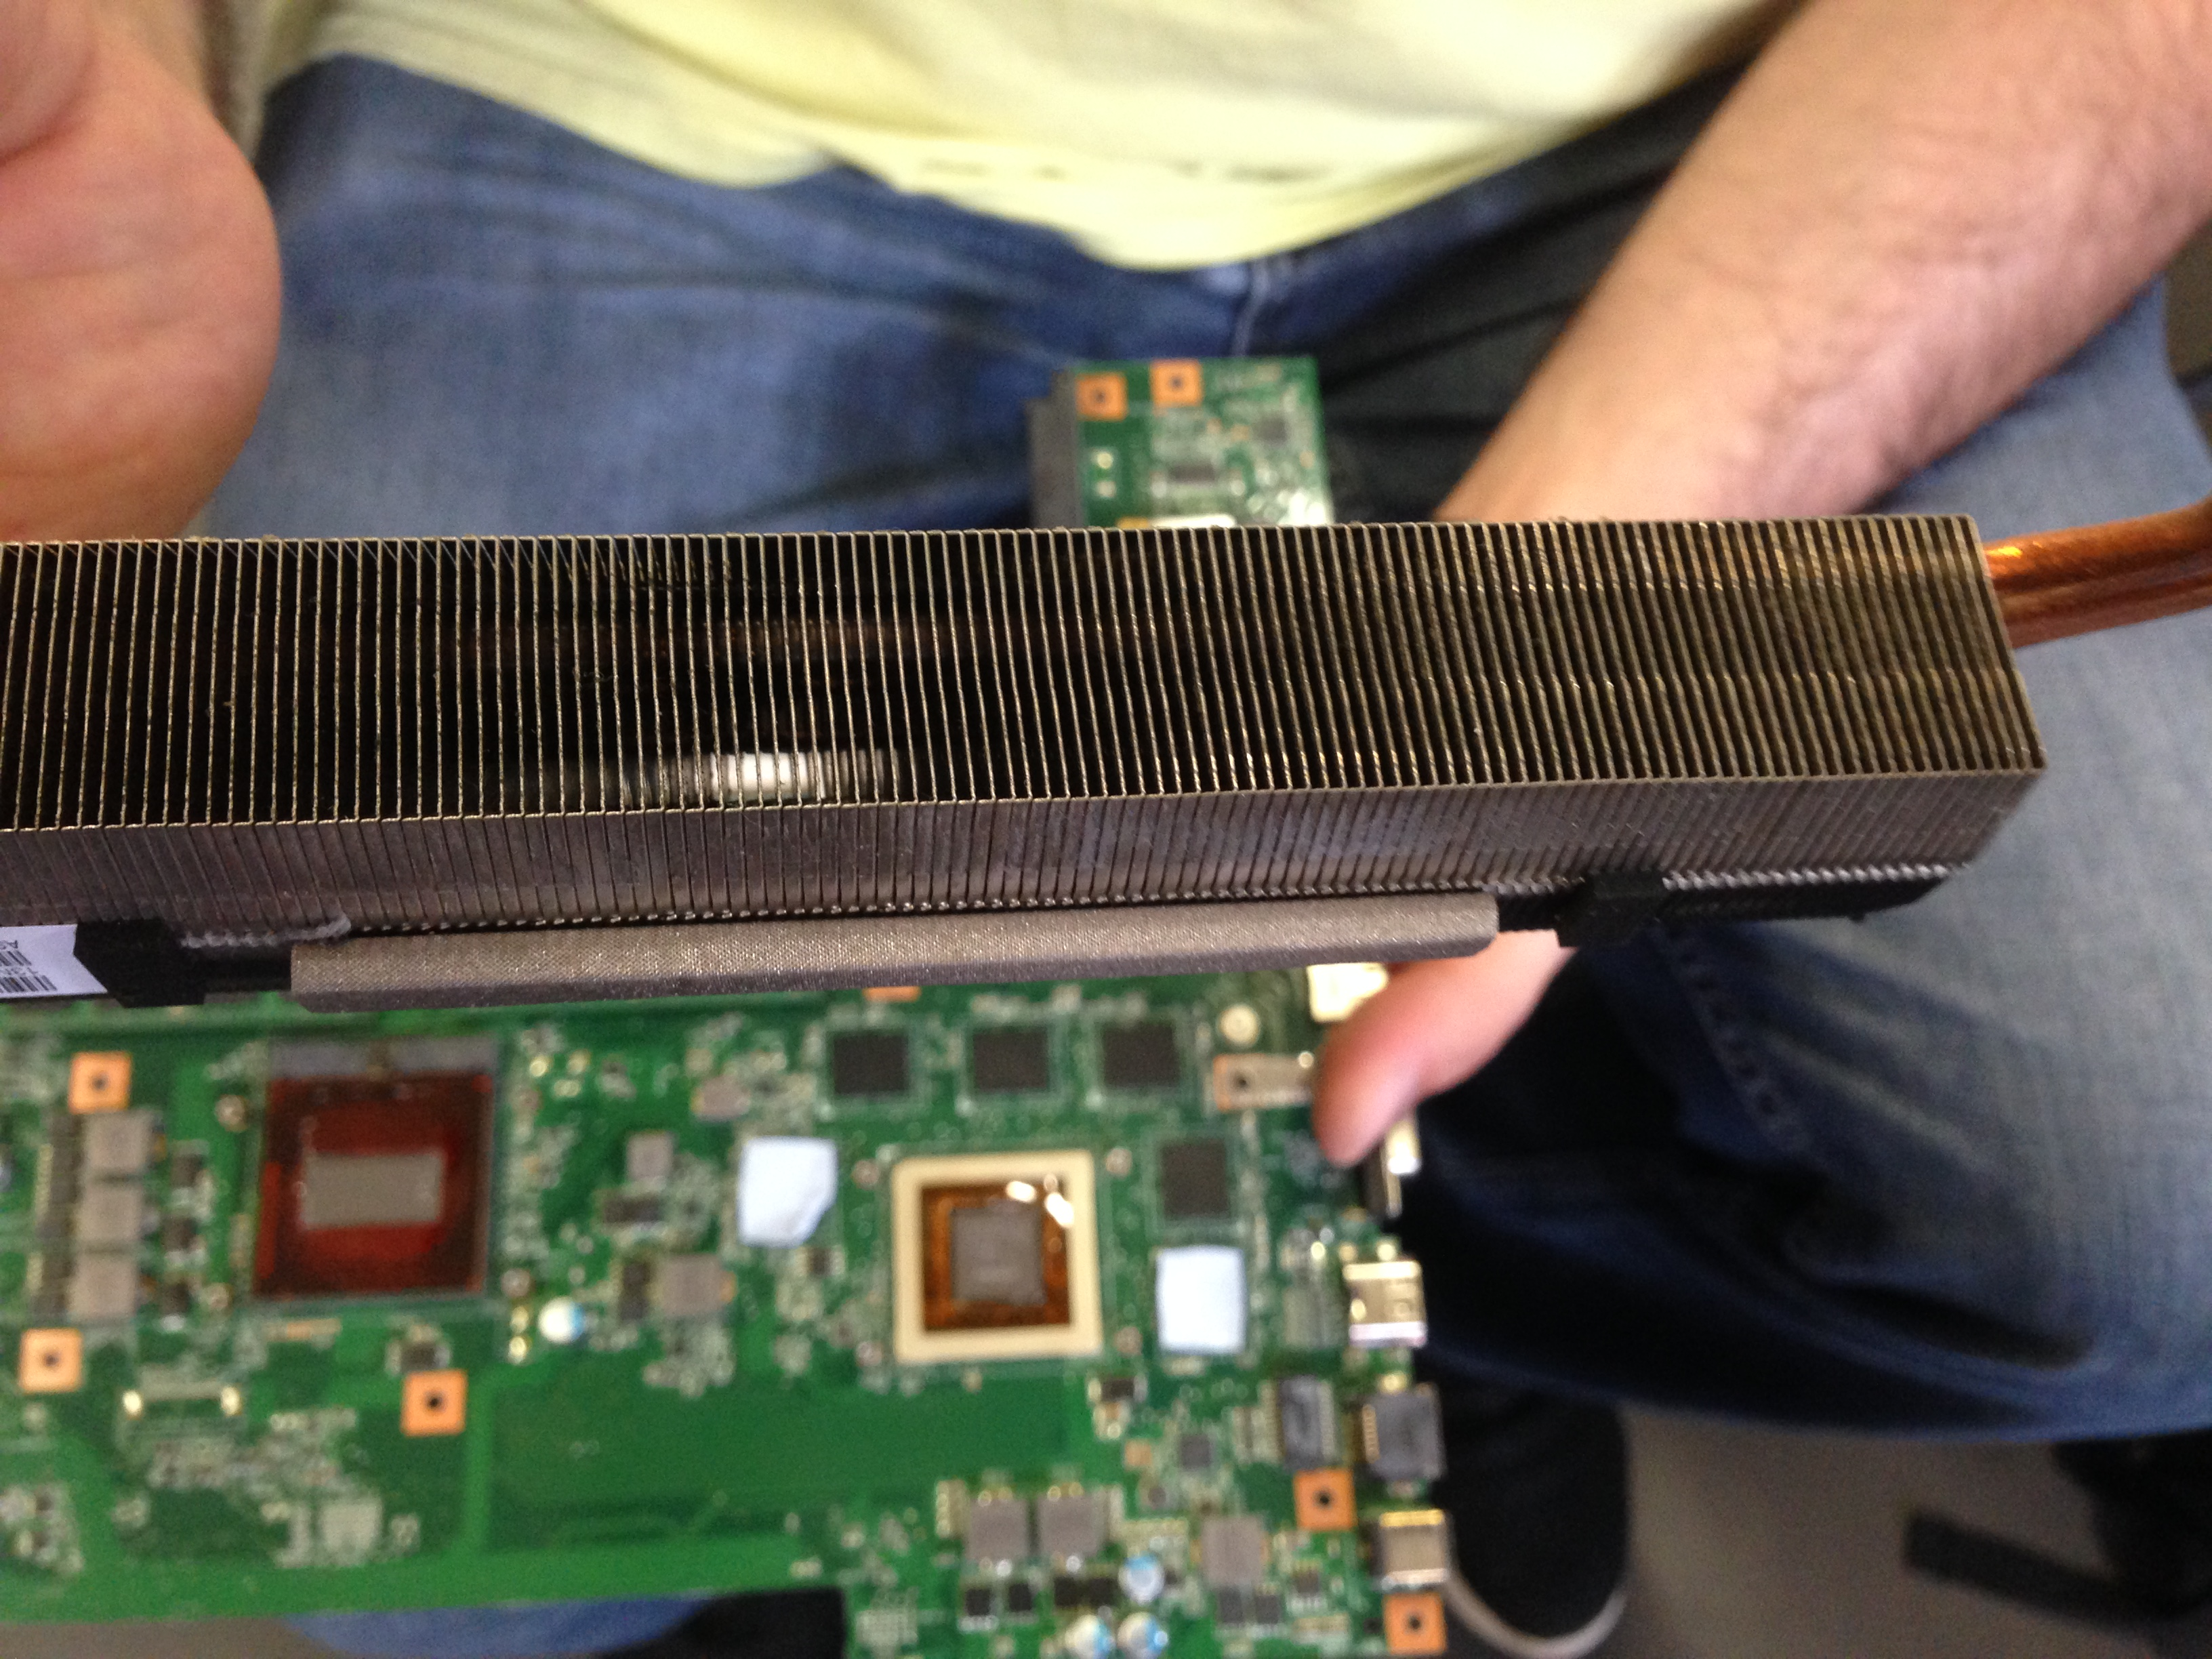
\includegraphics[scale=0.08]{cleaned-dust}
\end{frame}

\begin{frame}{Cleaned TIM}
    \centering
    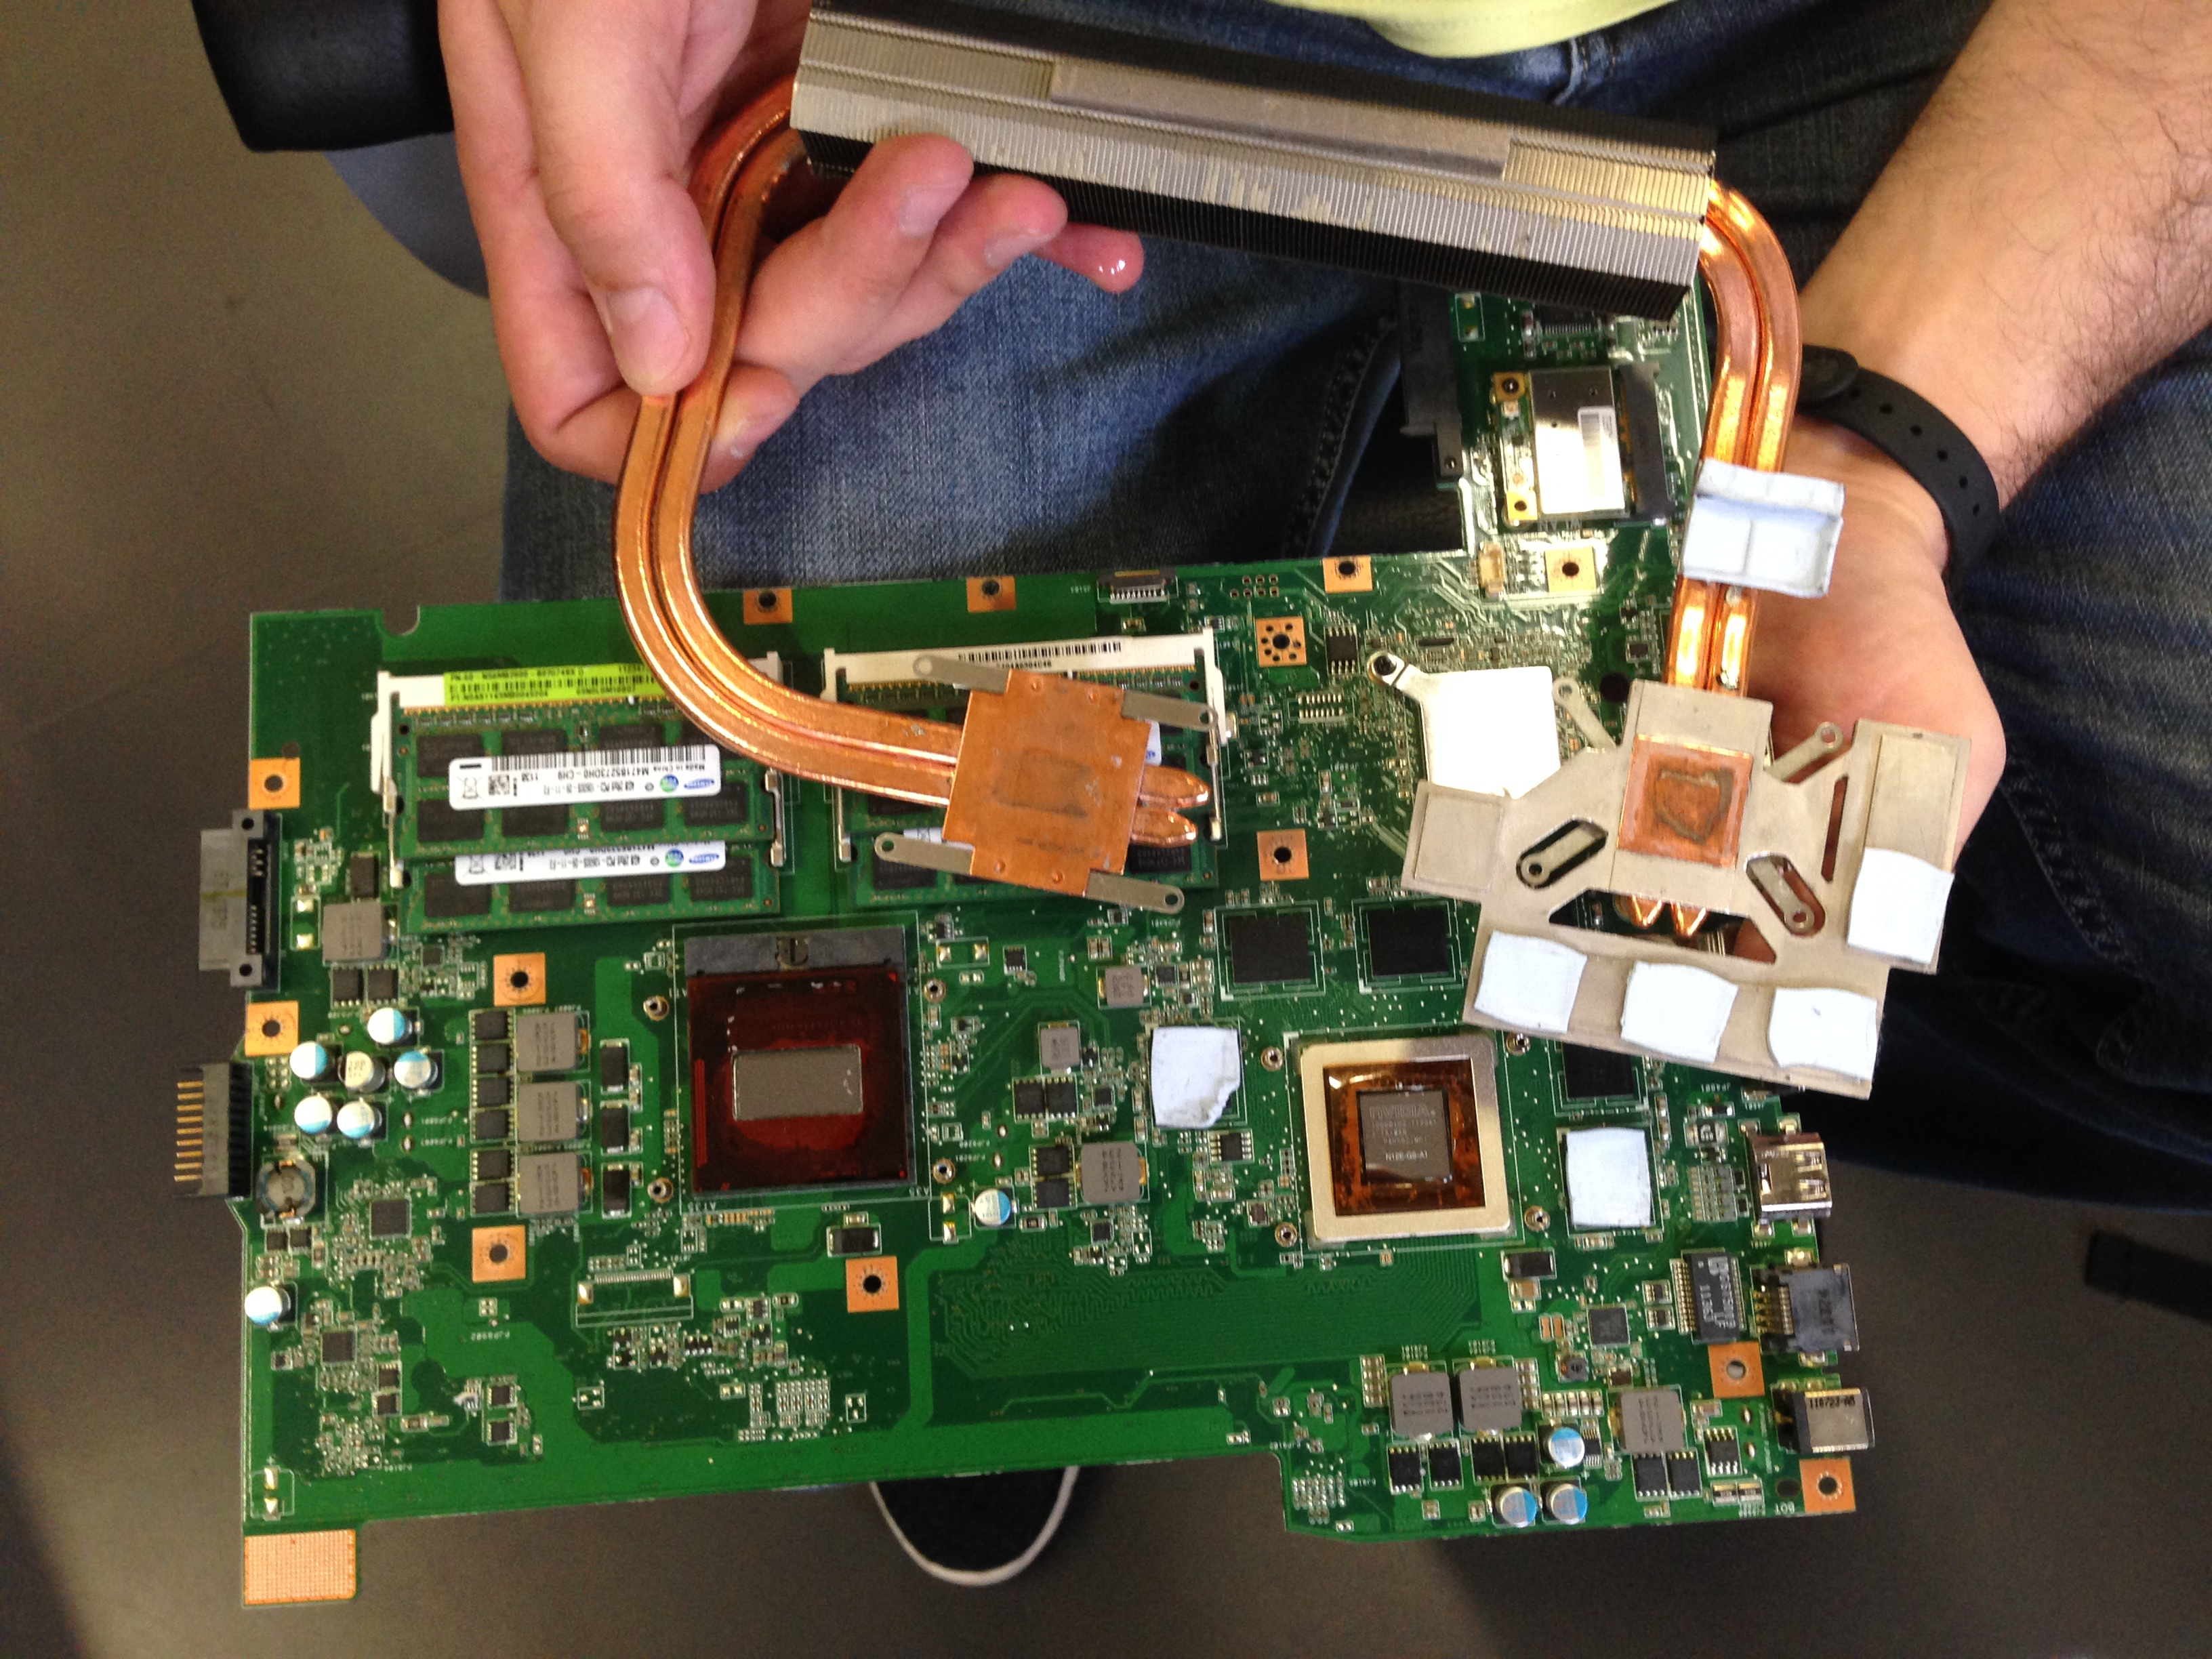
\includegraphics[scale=0.08]{cleaned-tim}
\end{frame}

\begin{frame}{Thermal Paste}
    \centering
    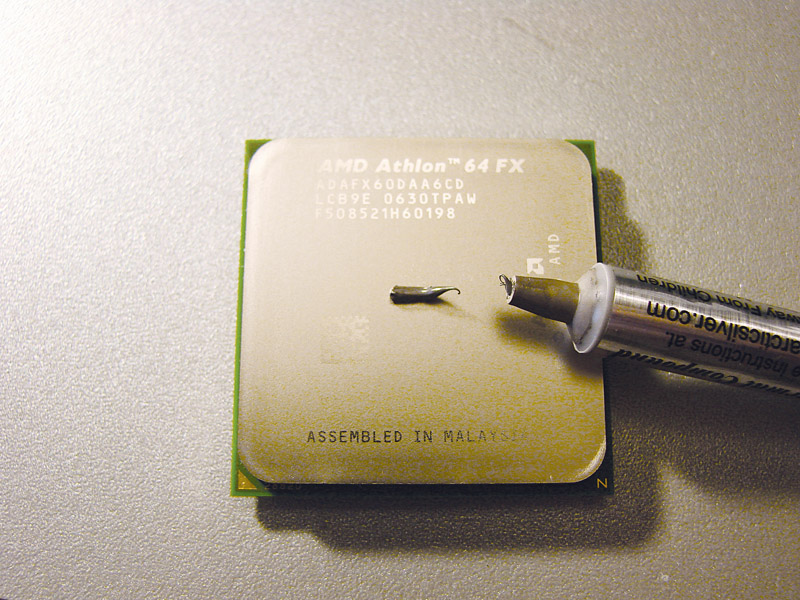
\includegraphics[scale=0.9]{tim-desktop-cpu}
\end{frame}

\begin{frame}{Thermal Paste}
    \centering
    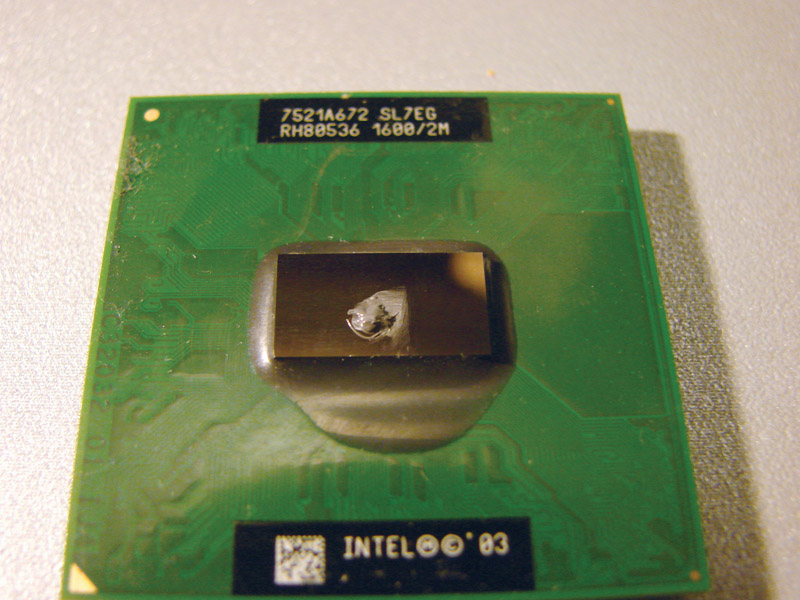
\includegraphics[scale=0.9]{tim-laptop-cpu}
\end{frame}

\begin{frame}{Thermal Paste}
    \centering
    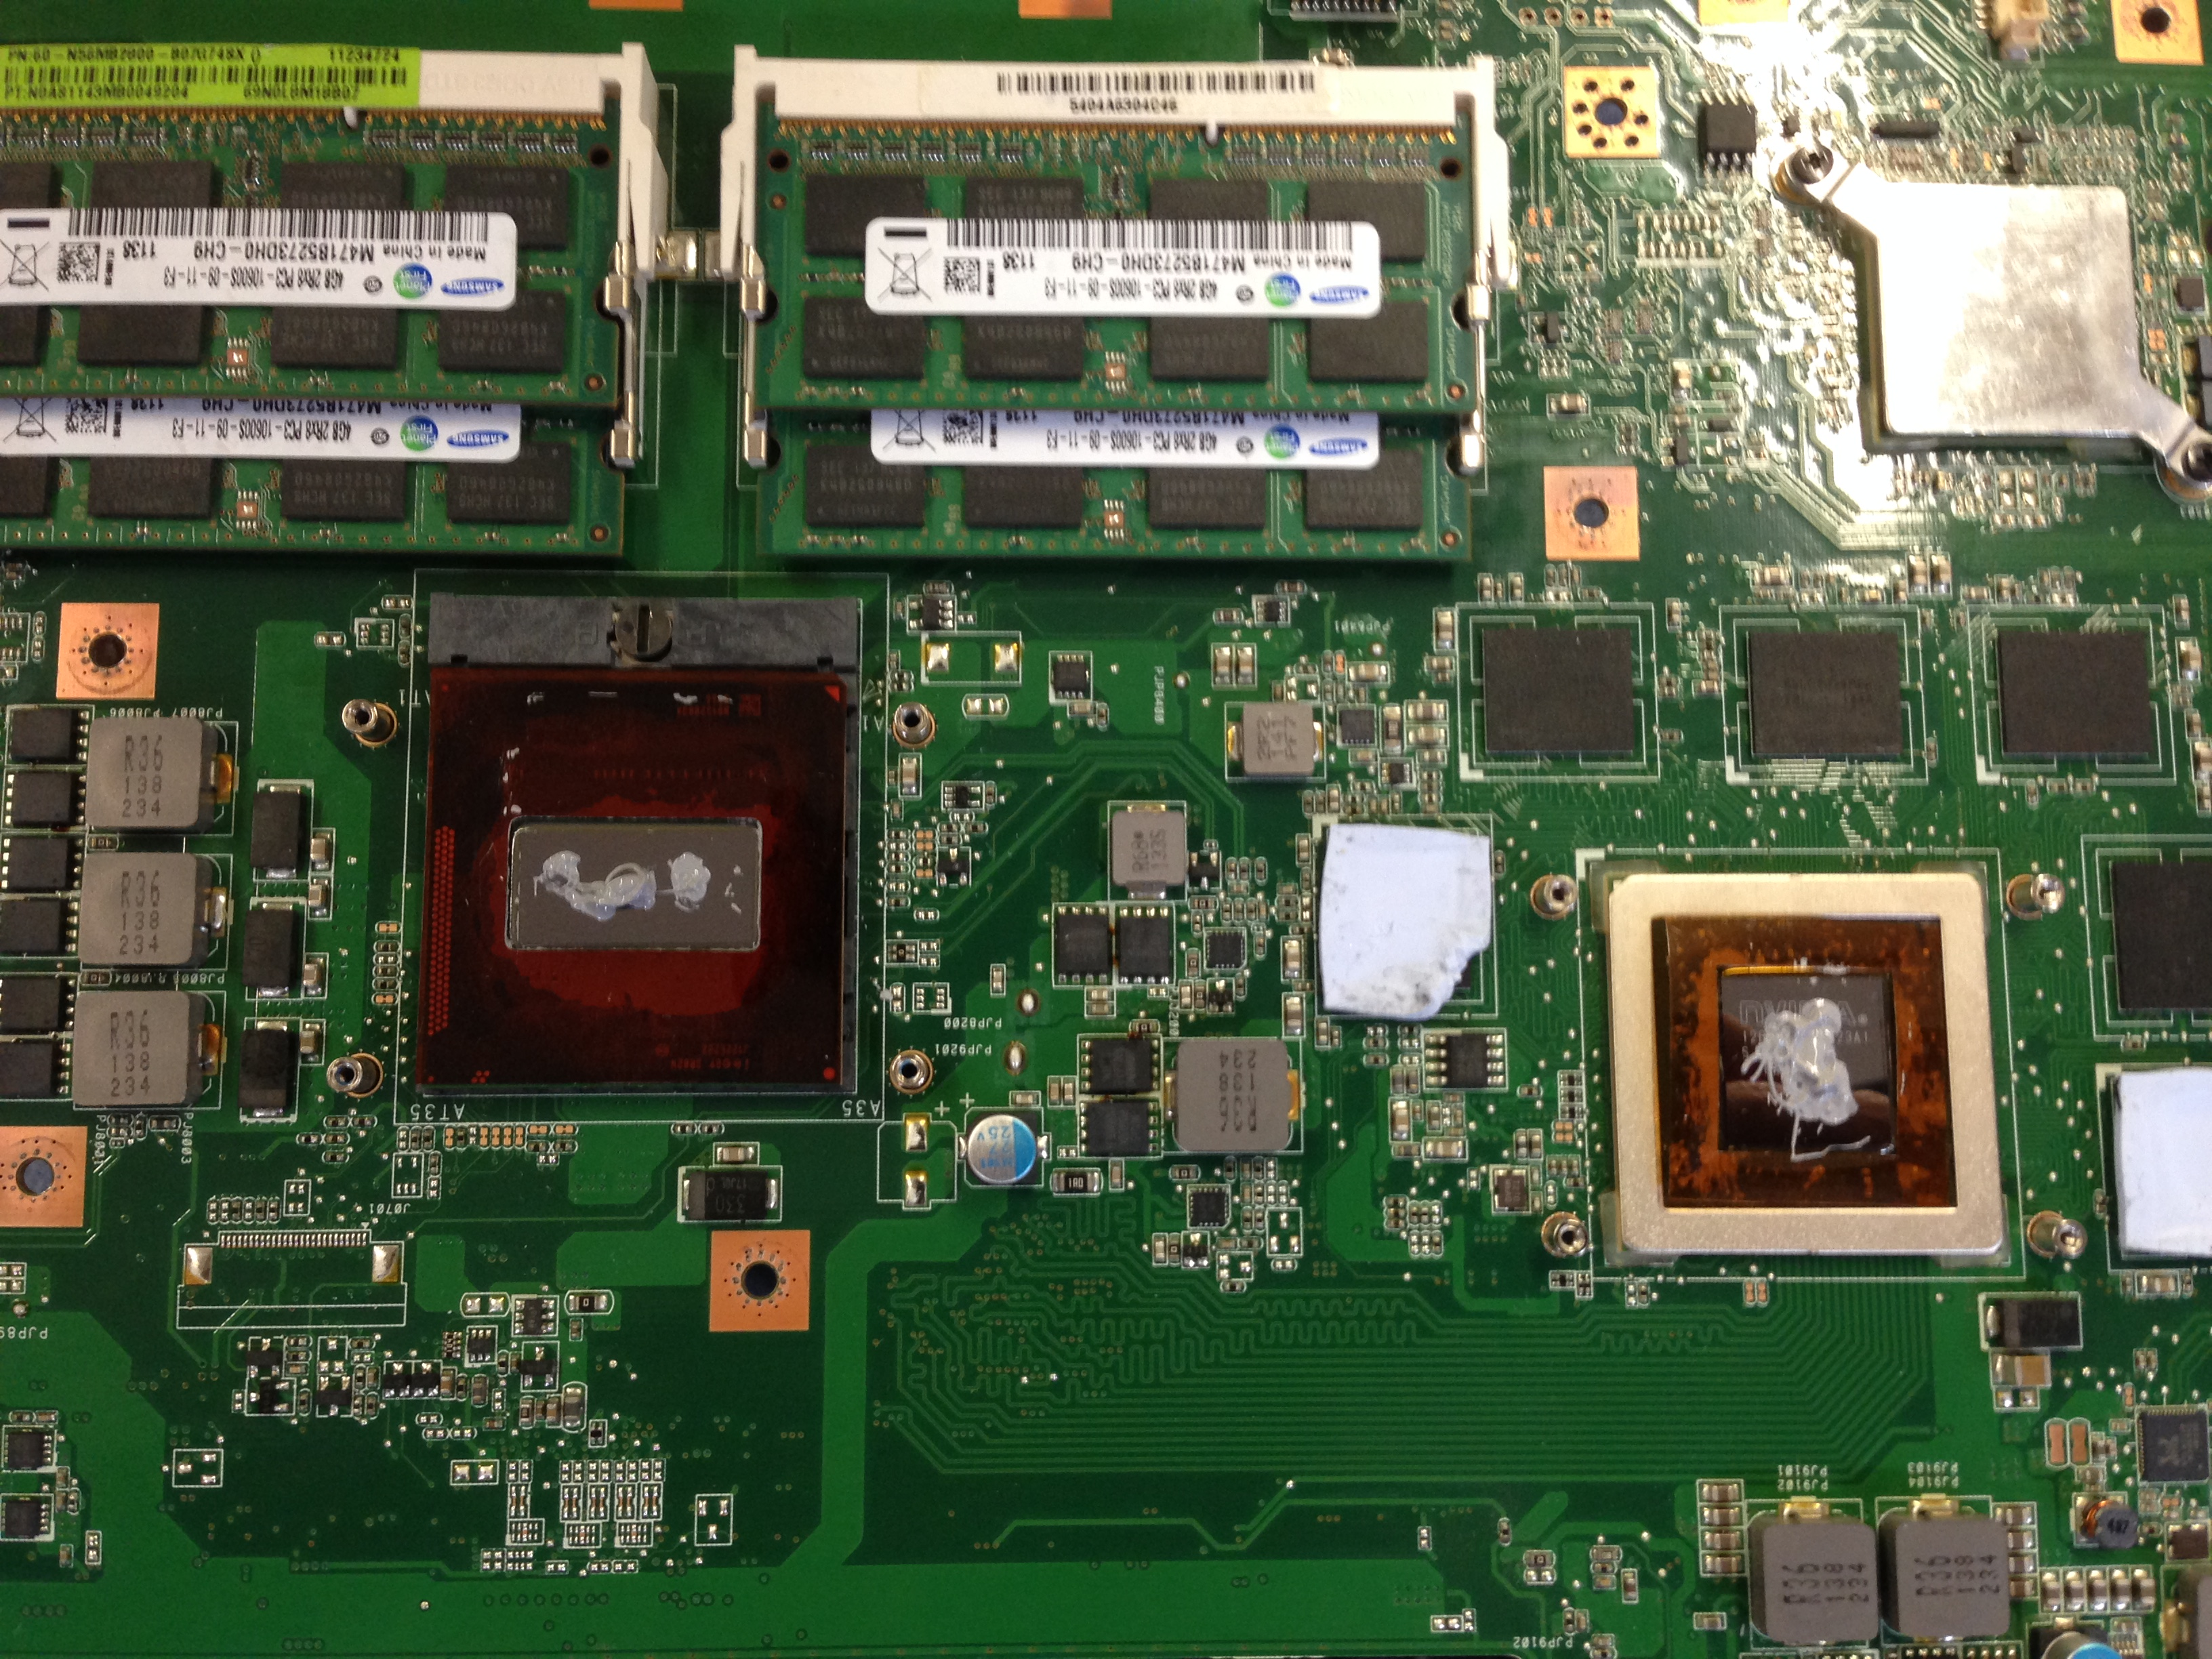
\includegraphics[scale=0.08]{tim-laptop-cpu-gpu}
\end{frame}

\begin{frame}{Assemble}
    \begin{itemize}
        \item Do it slowly
        \item Check if computer starts before closing it completely
        \item Check more than once that no screws and/or parts are forgotten
    \end{itemize}
\end{frame}

\section{Questions?}

\begin{frame}{Questions?}
    Go ahead, ask me anything (hardware related \textasciicircum\textasciicircum).
\end{frame}

\begin{frame}{Let's GO}
    \centering
    
\includegraphics[scale=0.25]{hands-on}
\end{frame}

\end{document}
